\chapter{Implementation} % Main chapter title

\label{Chapter6} % For referencing this chapter elsewhere, use \ref{Chapters}

\lhead{Chapter 6. \emph{Implementation}}

%----------------------------------------------------------------------------------------
%	SECTION 6.1
%----------------------------------------------------------------------------------------

\section{Frame}

This section comes after the literature review and requirements analysis to present the frame the software implementation will be developed on. This section will first go through the motivations in the choice of the frame as well as some perspective to move away from the objective and cover what will not be issued.

%-----------------------------------
%	SUBSECTION 6.1.1 - Motivations
%-----------------------------------

\subsection{Motivations}

Two objectives were set by missing information from the literature review. First, whether it is for development or acceleration frameworks, few benchmarks compare a similar implementation implemented in different frameworks. In terms of acceleration frameworks, this is due to the fact that few of them have opened their source code, making it time-consuming for one to perform a correct benchmark of the different frameworks. The other objective is to assess the importance of quantisation. While it has been proven that \emph{QNNs} could achieve the same accuracy and better throughput than classic \emph{CNNs}, few effort has been put in assessing the benefits and finding the best tailored precision for one's application.

Very few benchmarks exist on existing technologies, whether it is on development frameworks, or acceleration frameworks. The presentation of an accelerator often differs a lot from associated works and only state-of-the-art networks accuracy and throughputs are compared on simple architectures. Few projects seem to grow from the article they emerged from. \emph{YodaNN} \cite{Andri2016} does not provide any code outside of the article, neither does \emph{F-CNN} \cite{Zhao2016}. \emph{Tomato} \cite{Zhao2019}, \emph{TinyCNN} \cite{Jahanshahi2019} and \emph{fpgaConvNet} \cite{Venieris2017} face the same issue and make any comparison between the different frameworks very time-consuming. Only \emph{FINN} \cite{Umuroglu2017a, Blott2018} is still in active development and open-source.

Setting a benchmark from the open-source acceleration framework can help any external user have both a direct implementation of the framework as well as backed-up arguments on why it can help deploy one's application, at what cost and compared to state-of-the-art implementation. While the first objective presented earlier would be too time-consuming to complete, the second one is made possible through the usage of the open-source accelerator.

The main motivations taken in consideration when setting up the \emph{Brevitas} / \emph{FINN} benchmark is to provide an insight on the Xilinx tools and their workflow. This is important because widening the audience of the tool by presenting its capabilities allows both companies to be interested in the product as well as individuals to contribute to the project since it is open-source. The \emph{FINN} project started in September 2018 and has been in development ever since. The first version has been deprecated and a new direction is taken in 2019. The project is now using \emph{Brevitas} \cite{Pappalardo2020}, a PyTorch extension to perform the training and quantisation. \emph{FINN} is aiming at providing a clear acceleration of inference by deploying a network on an FPGA board. Both projects are open-source and can be found in their respective repositories on GitHub: \emph{FINN} \cite{FINNRepo} and \emph{Brevitas} \cite{BrevitasRepo}.

%--------------------------------------
%	SUBSECTION 6.1.2 - About Perspective
%--------------------------------------

\subsection{About Perspective}

Several papers present methods to \emph{train} networks on FPGAs \cite{Colangelo2018, Zhao2016, Jahanshahi2019}. However, while \emph{Brevitas} allows the training of \emph{QNNs}, it does not map the network on FPGAs at training time. It is expected to train the network on another hardware architecture (CPU(s) or GPU(s)) as PyTorch would expect and can handle. On the other hand, both \emph{Brevitas} and \emph{FINN} are in active development and in early phases of their development cycle. Version 0.3 of both tools has been released in late May this year.

%----------------------------------------------------------------------------------------
%	SECTION 6.2 - Workflow
%----------------------------------------------------------------------------------------

\section{Workflow}

This section will present the whole workflow \emph{Brevitas} / \emph{FINN} put into place. By first going through the \emph{QNN} designer and trainer that is \emph{Brevitas}, the quantised neural network is translated into the intermediate representation, \emph{ONNX}. The resulting intermediate representation can then be imported by \emph{FINN}. \emph{FINN} will perform several transformations and deploy part of the resulting graph on the associated FPGA.

%-----------------------------------
%	SUBSECTION 6.2.1 - Brevitas
%-----------------------------------

\subsection{Brevitas}

\emph{Brevitas} has been developed with the idea of corresponding to a \guille{drop-in} replacement of PyTorch. This means that it ensures that PyTorch functionalities will be kept, even when working with reduced-precision layers. \emph{Brevitas} implements a set of building blocks to model a reduced precision hardware data-path at training time. While partially biased towards modelling data-flow-style, very low-precision implementations, the building blocks can be parametrised and assembled together to target all sorts of reduced precision hardware.

The implementation sets up several design principles: idiomatic PyTorch if possible, modularity first at the cost of some verbosity and a focus on easy extendability. \emph{Brevitas} features many different ideas such as extracted from its presentation:
\begin{itemize}
  \item \textbf{Quantisation Type}: Binary, ternary or uniform integer.
  \item \textbf{Target Tensor}: Weights, activations or accumulators.
  \item \textbf{Scaling}: Support for different shapes, learning strategies and constraints.
  \item \textbf{Precision}: Constant or learned bit-width.
  \item \textbf{Cost}: Hardware cost modelled at training time.
\end{itemize}

Note that \emph{scaling} is the method used by \emph{Brevitas} to preserve a good precision even though the layers use quantised parameters. \emph{Brevitas} handles several different methods to determine the scaling factor. It determines it either with respect to the number of dimensions, with respect to a learned parameter, shared between different layers or constrained to specific values. On the other hand, \emph{Brevitas} supports both constant and learned precision.

As an example, we would like to define the \emph{LeNet-5} architecture as presented by Le Cun et al. \cite{LeCun1998}. The \emph{PyTorch} version can be seen on \emph{Figure} \ref{fig:LeNetPyTorch}. It consists of an extension of the \texttt{Module} class. The layers are then defined into two separate parts in the initialisation method. In one side and as part of a \texttt{Sequential}, the layers performing the \emph{feature extraction}. Those layers consist mostly of convolutions, pooling and activations, sometimes with batch normalisations and dropouts. In our case, the \emph{feature extraction} consists of three sequences of \texttt{Convolution => TanH Activation => Average Pooling}. Next comes the \emph{classifier} sequence, represented by a \texttt{Sequential} as well. It consists of fully-connected layers and end up with a number of neurons equal to the number of classes. Here, our \emph{classifier} consists of two fully-connected layers.

PyTorch asks to define the \texttt{function} and manages backpropagation on its own when dealing with a neural network. Here, the forward function consists of feeding the instance (image supposedly) in the \emph{feature extractor}, reshaping the result into a 1-dimensional array, feeding this array to the \emph{classifier} and using a \emph{softmax} function to access the probabilities determined for each of the classes of the dataset.

% PyTorch LeNet5 implementation
\begin{figure}[htbp]
\centering
\begin{lstlisting}[language=Python]
import torch
import torch.nn as nn
import torch.nn.functional as F

class LeNet5(nn.Module):
  '''LeNet5 architecture in PyTorch'''
  def __init__(self, n_classes=10, in_channels=3):
    super(LeNet5, self).__init__()

    self.feature_extractor = nn.Sequential(
      nn.Conv2d(in_channels=in_channels, out_channels=6,
                kernel_size=5, stride=1),
      nn.Tanh(),
      nn.AvgPool2d(kernel_size=2),
      nn.Conv2d(in_channels=6, out_channels=16,
                kernel_size=5, stride=1),
      nn.Tanh(),
      nn.AvgPool2d(kernel_size=2),
      nn.Conv2d(in_channels=16, out_channels=120,
                kernel_size=5, stride=1),
      nn.Tanh()
    )

    self.classifier = nn.Sequential(
      nn.Linear(in_features=120, out_features=84),
      nn.Tanh(),
      nn.Linear(in_features=84, out_features=n_classes),
    )

    self.name = "LeNet5"

  def forward(self, x):
    out = self.feature_extractor(x)
    out = out.view(out.size(0), -1)
    out = self.classifier(out)
    return F.softmax(out, dim=1)
\end{lstlisting}
\caption[LeNetPyTorch]{PyTorch LeNet-5 \cite{LeCun1998} implementation}
	\label{fig:LeNetPyTorch}
\end{figure}


On the other hand, \emph{Brevitas} provides a very similar API in terms of layer definition. The one thing changing is the need to specify the bit-width, or precision, of each one of the layers. In the example, the bit-width is determined from three parameters at initialisation: \texttt{weight\_bit\_width}, the bit-width used for the weights parameters ; \texttt{act\_bit\_width}, the bit-width used for the activations and \texttt{in\_bit\_width}, the bit-width used for the input layer. This last bit-width is important because the first layer is particularly sensible to precision changes and often requires a higher-precision to not deteriorate too much the end accuracy. An example of the \emph{Brevitas} way to define \emph{LeNet-5} is presented in \emph{Figure} \ref{fig:LeNetBrevitas}.


\begin{figure}[htbp]
\centering
\begin{lstlisting}[language=Python]
import torch
import \emph{Brevitas}.nn as bnn
import torch.nn.functional as F

class QuantLeNet5(nn.Module):
  '''LeNet5 architecture in PyTorch'''
  def __init__(self, n_classes=10, in_channels=3,
           weight_bit_width=4, act_bit_width=4, in_bit_width=8):
    super(QuantLeNet5, self).__init__()

    self.feature_extractor = nn.Sequential(
      bnn.QuantConv2d(in_channels = in_channels, out_channels = 6,
                      kernel_size = 5, stride = 1,
                      bit_width = in_bit_width),
      bnn.QuantTanh(bit_width = act_bit_width),
      bnn.QuantAvgPool2d(kernel_size=2, bit_width = weight_bit_width),
      bnn.QuantConv2d(in_channels=6, out_channels=16,
                      kernel_size=5, stride=1,
                      bit_width = weight_bit_width),
      bnn.QuantTanh(bit_width = act_bit_width),
      bnn.QuantAvgPool2d(kernel_size=2, bit_width = weight_bit_width),
      bnn.QuantConv2d(in_channels=16, out_channels=120,
                      kernel_size=5, stride=1,
                      bit_width = weight_bit_width),
      bnn.QuantTanh(bit_width = act_bit_width)
    )

    self.classifier = nn.Sequential(
      bnn.QuantLinear(in_features=120, out_features=84,
                      bit_width = weight_bit_width),
      bnn.QuantTanh(bit_width = act_bit_width),
      bnn.QuantLinear(in_features=84, out_features=n_classes,
                      bit_width = weight_bit_width),
    )

    self.name = "QuantLeNet5"

  def forward(self, x):
    out = self.feature_extractor(x)
    out = out.view(out.size(0), -1)
    out = self.classifier(out)
    return F.softmax(out, dim=1)
\end{lstlisting}
\caption[LeNetBrevitas]{Brevitas quantised LeNet-5 \cite{LeCun1998} implementation}
	\label{fig:LeNetBrevitas}
\end{figure}

Once the neural network is defined and trained, \emph{Brevitas} provides a way to export it to the intermediate representation. This representation is the focus of the next subsection and will be looked into in more details later on. \emph{Brevitas} uses specific annotations to define the quantised layers.  The intermediate representation, called \emph{ONNX} does not provide a way to represent layers with precisions under 8-bit. This is why this system of custom annotations has been created. These specific annotations can then be used by \emph{FINN} to perform transformations on.

%--------------------------------------
%	SUBSECTION 6.2.2 - ONNX
%--------------------------------------

\subsection{ONNX}

As extracted from their repository: \guille{\emph{Open Neural Network Exchange (ONNX)} is an open ecosystem that empowers AI developers to choose the right tool for their project}. \emph{ONNX} provides an open-source format for artificial intelligence and machine learning models. This is done by defining an extensible computation graph model, as well as definitions of operators and data types. \emph{ONNX} is widely supported in different frameworks or tools. The main goal behind its design and development was to \guille{enable interoperability between different frameworks to streamline the path between research and production} \cite{ONNXRepo}.

\emph{Figure} \ref{fig:ONNXBeginning} presents the \emph{ONNX} representation of a network architecture called \emph{TFC} and corresponding to three fully-connected layers put one after each other. This \emph{ONNX} representation is obtained through the export modules in \emph{Brevitas}, and particularly \texttt{brevitas.onnx}. This module is still under active development by the Xilinx team. The visualisation is made possible through the \emph{Netron} tool \cite{NetronRepo}.

% TFC \emph{ONNX} THROUGH NETRON
\begin{figure}[htbp]
	\centering
		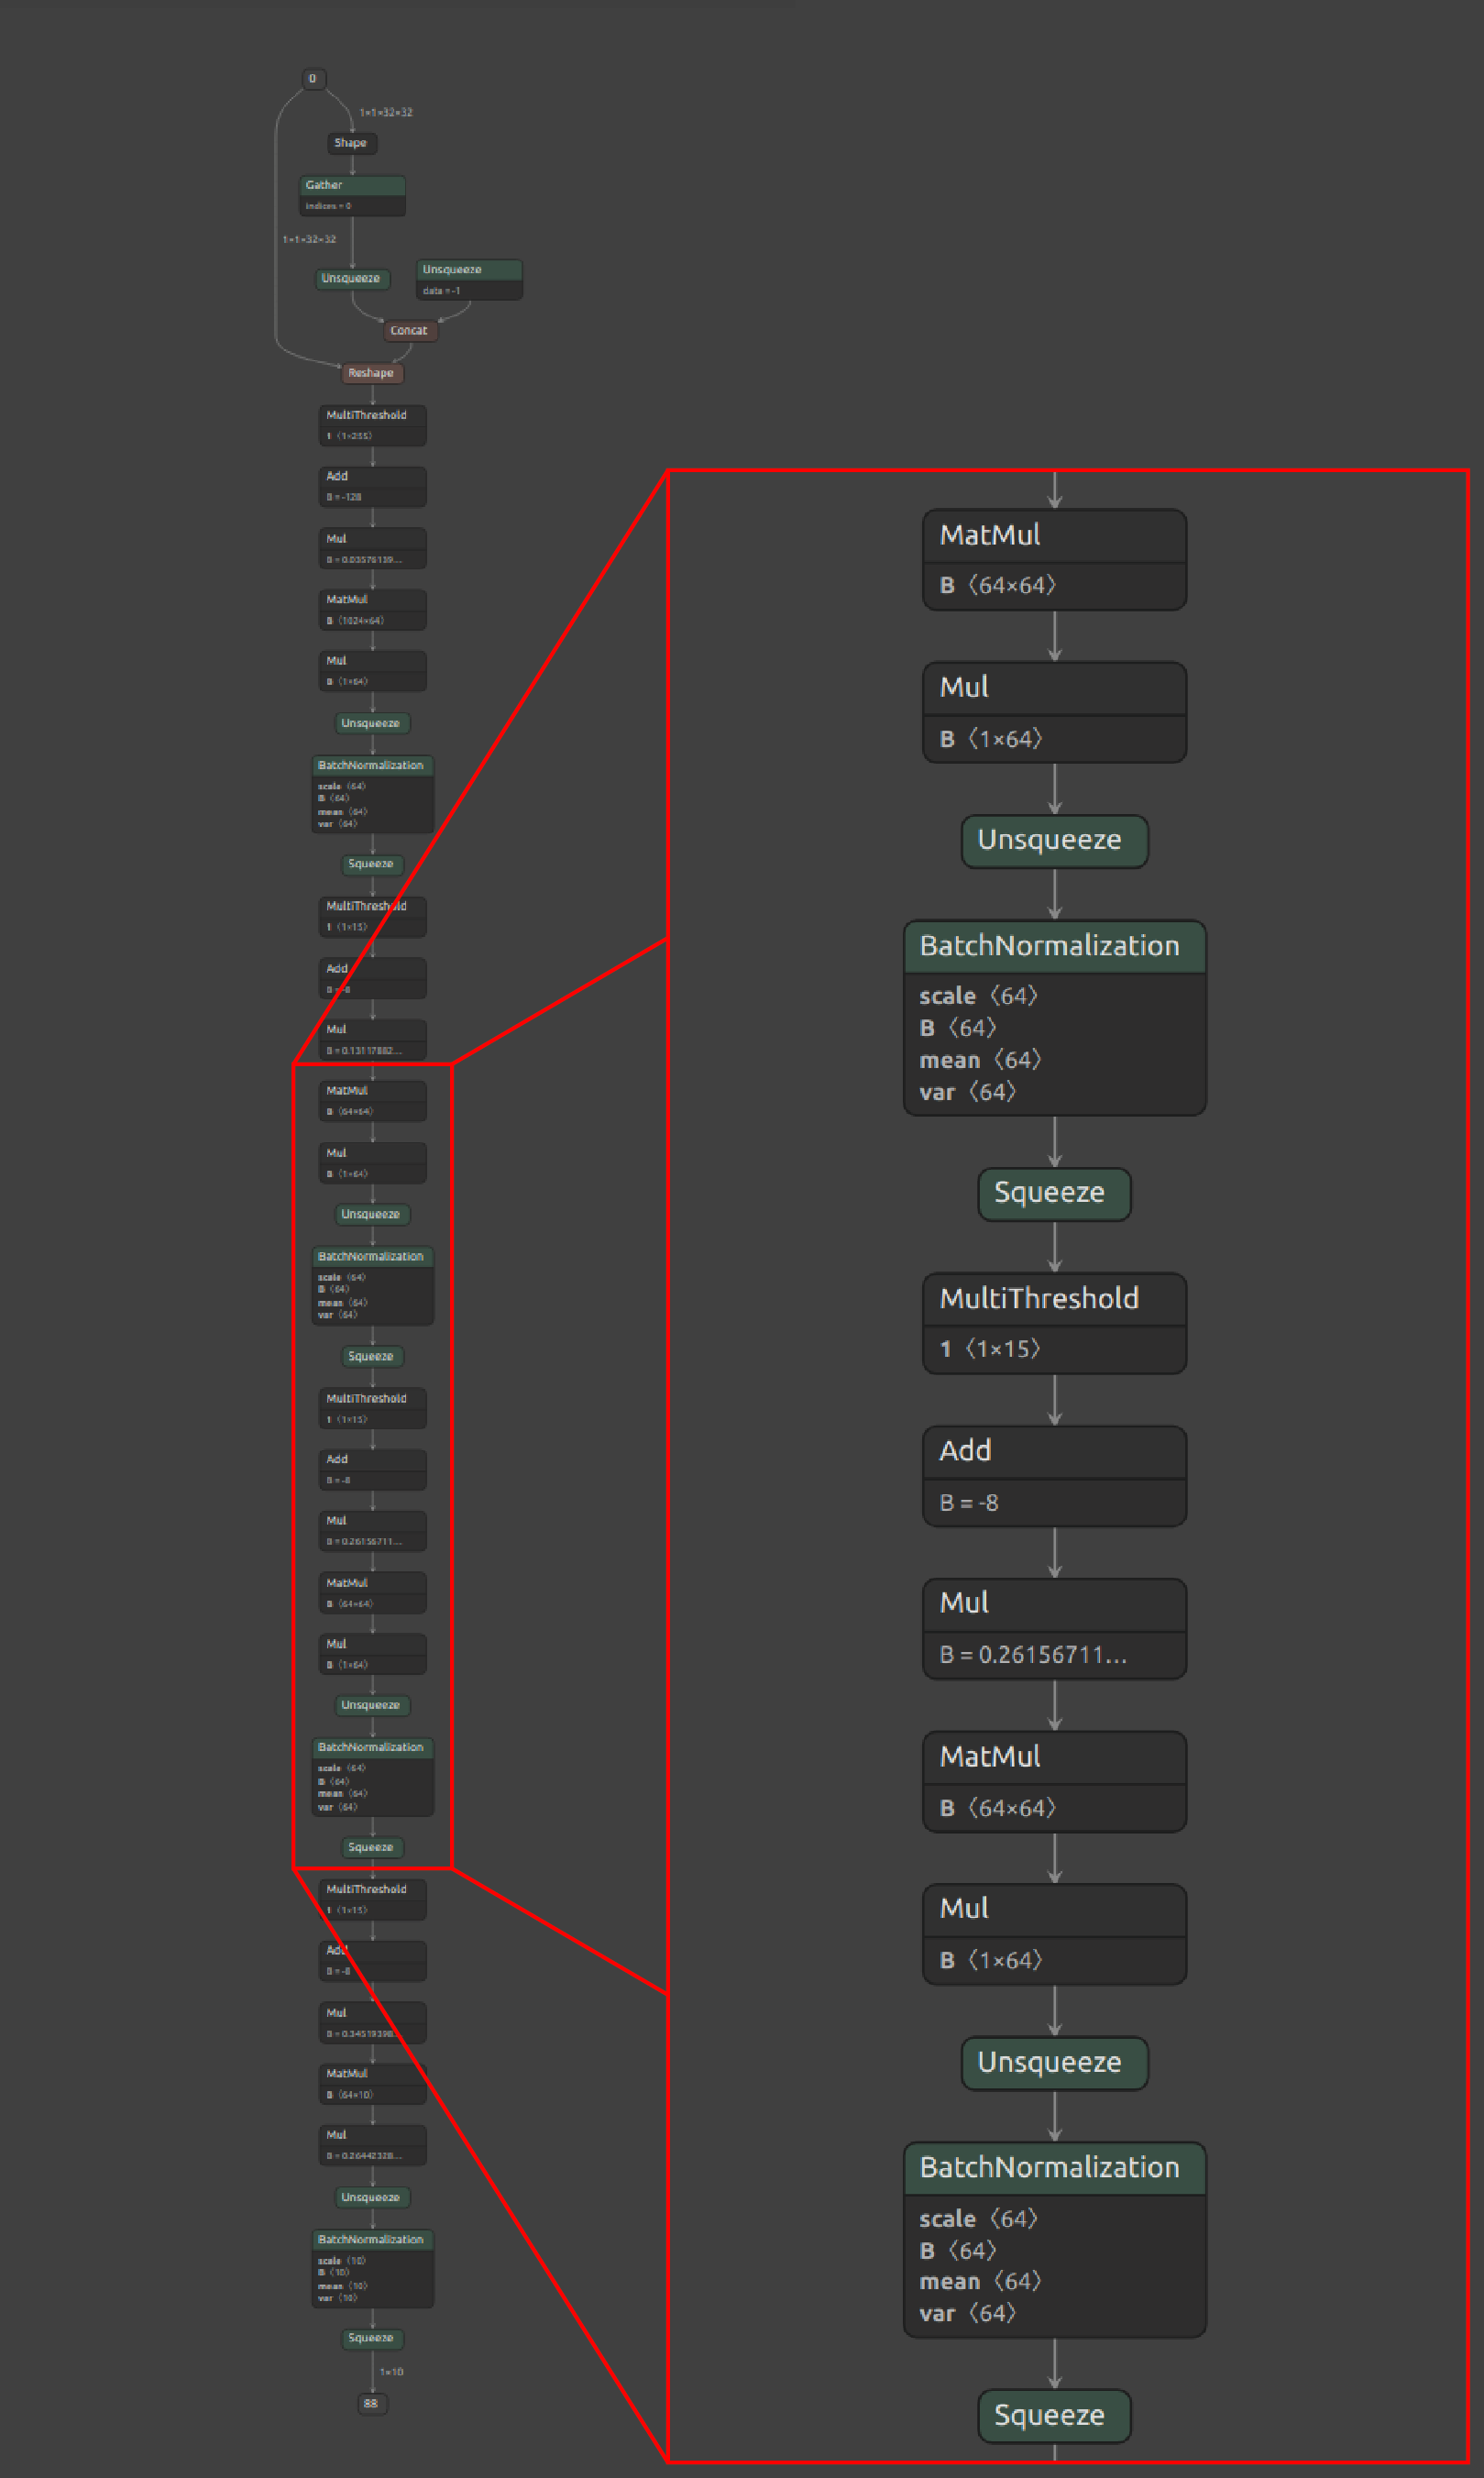
\includegraphics[width=12cm]{Figures/ONNXBeginning.png}
	\caption[TFC \emph{ONNX} representation]{TFC \emph{ONNX} Representation}
	\label{fig:ONNXBeginning}
\end{figure}

\newpage

%-------------------------
%	SUBSECTION 6.2.3 - FINN
%-------------------------

\subsection{FINN}

The last piece of the workflow is \emph{FINN}, described by Xilinx as allowing \guille{Fast, Scalable Quantized Neural Network Inference on FPGAs}. The \emph{FINN} compiler goes through three major steps to be able to port a neural network as shown on \emph{Figure} \ref{fig:FINNWholeFlow}. First, \emph{Network Preparation} where \emph{FINN} uses different transformations on the \emph{ONNX} graph to simplify it or make it more convenient for the next steps. Then, \emph{IP Generation} where the \emph{Vivado} tool is called to generate a network of HLS layers with one IP block per layer and finally stitches all the blocks together. Finally, the network is deployed on an FPGA with a \emph{PYNQ} shell, an FPGA utility providing a Python environment on an FPGA. This deployment is made possible by creating a project and driver then transferring it on the board along with the bitfile.

% \emph{FINN} WHOLE FLOW
\begin{figure}[htbp]
	\centering
		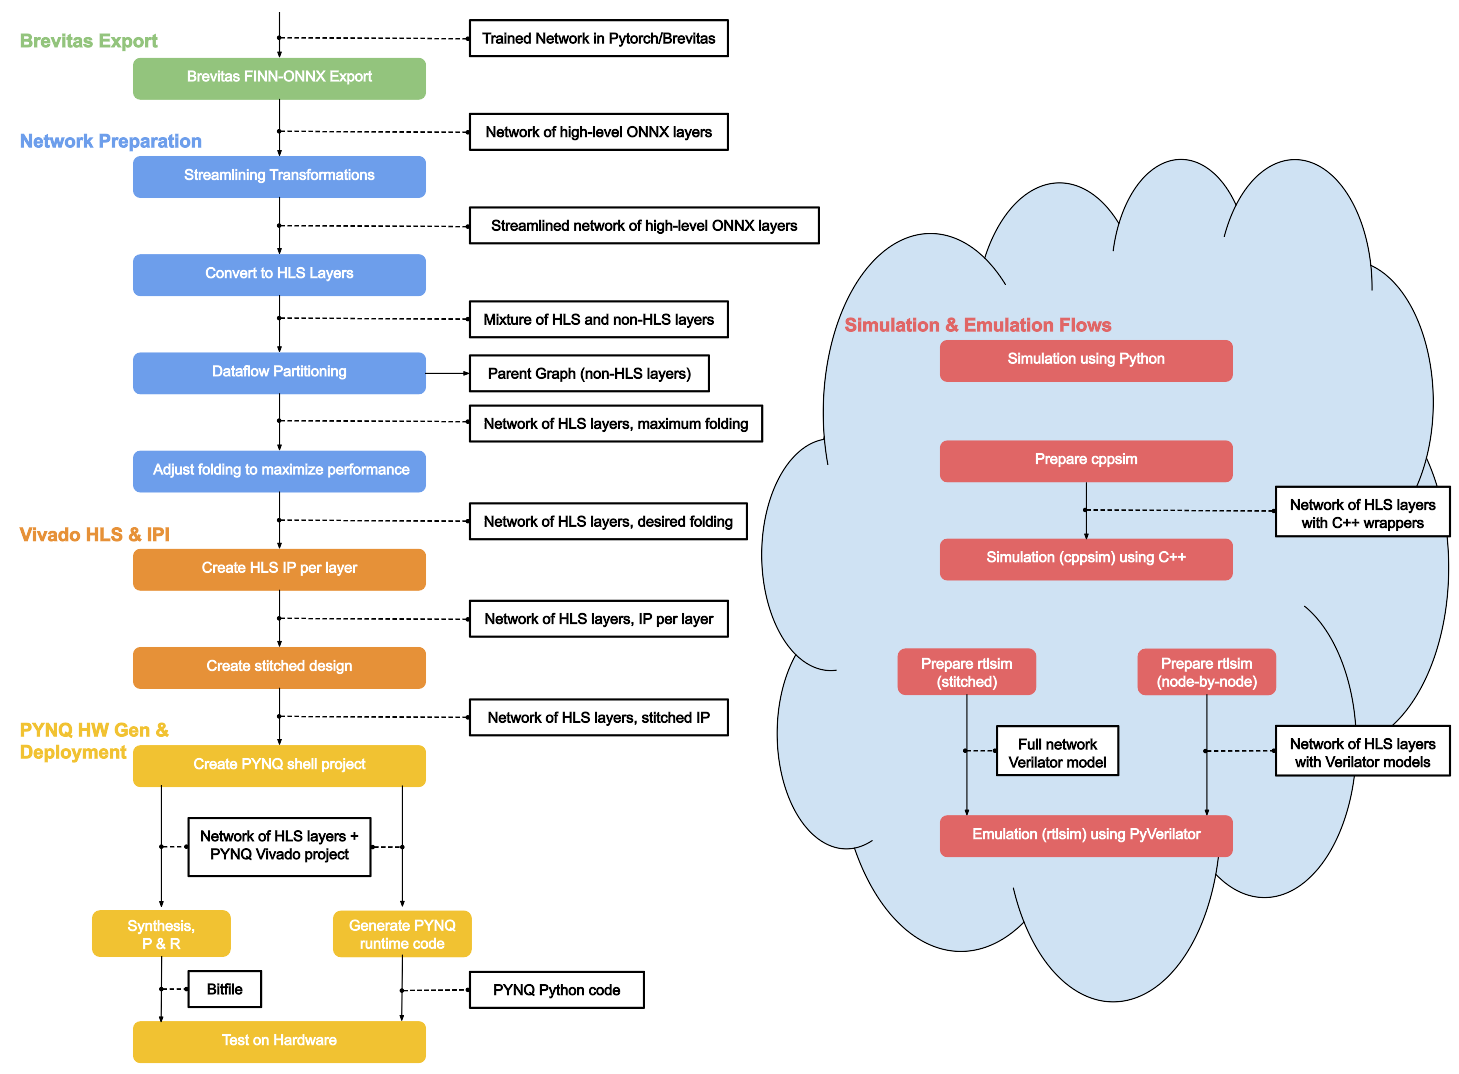
\includegraphics[width=16cm]{Figures/FINNWholeFlow.png}
	\caption[FINN whole flow]{FINN workflow from \emph{Brevitas} import to FPGA deployment}
	\label{fig:FINNWholeFlow}
\end{figure}

% \emph{FINN} TRANSFORMATIONS
\begin{figure}[htbp]
	\centering
		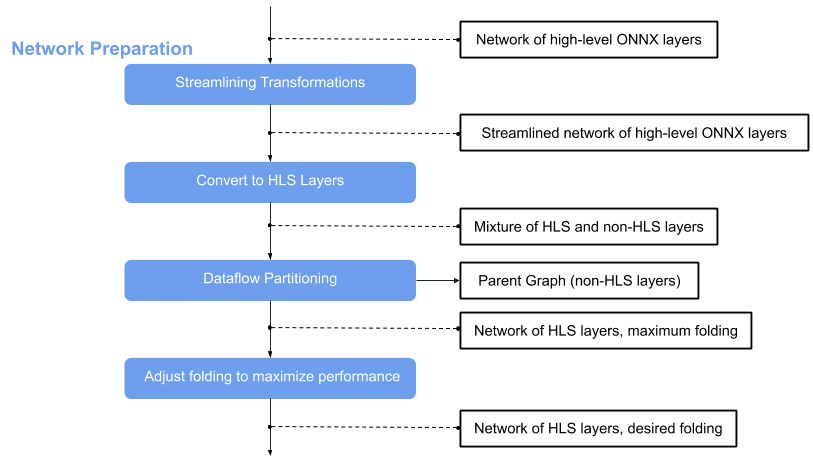
\includegraphics[width=8cm]{Figures/FINNTransformations.png}
	\caption[FINN Transformations]{FINN Transformations}
	\label{fig:FINNTransformations}
\end{figure}

The network preparation part is the one involving several transformations in the structure of the neural network graph. The transformations are separated in three categories: tidy-up, streamlining, HLS conversion and dataflow partition. All the different transformations, whether they are used for tidy-up or synthesis purposes, are applied on a \texttt{ModelWrapper}. The flow of transformations can be seen on \emph{Figure} \ref{fig:FINNTransformations}.

\emph{Tidy-up Transformations} consist of renaming the nodes so they have unique names, checking the data type and shapes of the tensors used. Examples of these different transformations are \texttt{GiveReadableTensorNames}, \texttt{GiveUniqueNodeNames} or \texttt{InferShapes}.

\emph{Streamline Transformations} consist of a way to remove floating-point operations from the graph. The streamlining process itself contains three steps:
\begin{itemize}
  \item \textbf{Successive Thresholding}: Given a set of threshold values, the successive thresholding function maps any real number $x$ to an integer corresponding to the number of thresholds $x$ is greater or equal to. This way, any uniform quantifier can be expressed as successive thresholding followed by a linear transformation: $Q(x) = a*T(x) + b$.
  \item \textbf{Collapsing Linear Transformation}: All \emph{floating point} linear operations are positioned between the quantised matrix operation and the activation quantisation. Any sequence of linear transformation can be collapsed in a single linear transformation.
  \item \textbf{Absorbing into Thresholds} :Updating the threshold values with the changes in the linear transformations removes any linear transformation from the graph.
\end{itemize}

The \texttt{Streamline} transformation class is implemented as presented on \emph{Figure} \ref{fig:FINNStreamline}.

\begin{figure}[htbp]
\centering
\begin{lstlisting}[language=Python]
class Streamline(Transformation):
  """Apply the streamlining transform, see arXiv:1709.04060."""

  def apply(self, model):
    streamline_transformations = [
      ConvertSubToAdd(),
      ConvertDivToMul(),
      BatchNormToAffine(),
      ConvertSignToThres(),
      MoveAddPastMul(),
      MoveScalarAddPastMatMul(),
      MoveScalarAddPastConv(),
      MoveScalarMulPastMatMul(),
      MoveScalarMulPastConv(),
      MoveAddPastMul(),
      CollapseRepeatedAdd(),
      CollapseRepeatedMul(),
      AbsorbAddIntoMultiThreshold(),
      FactorOutMulSignMagnitude(),
      AbsorbMulIntoMultiThreshold(),
      Absorb1BitMulIntoMatMul(),
      Absorb1BitMulIntoConv(),
      RoundAndClipThresholds(),
    ]
    for trn in streamline_transformations:
      model = model.transform(trn)
      model = model.transform(GiveUniqueNodeNames())
      model = model.transform(GiveReadableTensorNames())
      model = model.transform(InferDataTypes())
    return (model, False)
\end{lstlisting}
\caption[FINN Streamline]{FINN Streamline process as proposed in \cite{Umuroglu2017b, Blott2018}}
	\label{fig:FINNStreamline}
\end{figure}

\newpage

Once the streamlining transformations are completed, \emph{FINN} will convert the different layers to their HLS counterpart if possible. This conversion is made possible by using \texttt{finn-hls}, a backend library developed by the same team to translate layers to HLS. The result of the transformation consists of a mixture of HLS and non-HLS layers. The \emph{HLS Conversion} completed, \emph{FINN} will then proceed to a \emph{Dataflow Partitioning}. This step will separate the whole network graph into a parent graph that will be executed through the \texttt{onnx-exec}. One of its child node contains all the different HLS layers and during the execution of the whole graph, \emph{FINN} delegates the execution of this child node to the FPGA board and gets the result before injecting it back in the graph execution flow. The resulting \emph{ONNX} representation can be seen on \emph{Figure} \ref{fig:ONNXEnd} where the network and its \emph{ONNX} representation (presented earlier on \emph{Figure} \ref{fig:ONNXBeginning}) now corresponds to few basic operations followed by a \texttt{StreamingDataflowPartition} layer that contains the layers that need to be deployed.

\newpage

% END TFC \emph{ONNX} THROUGH NETRON
\begin{figure}[htbp]
	\centering
		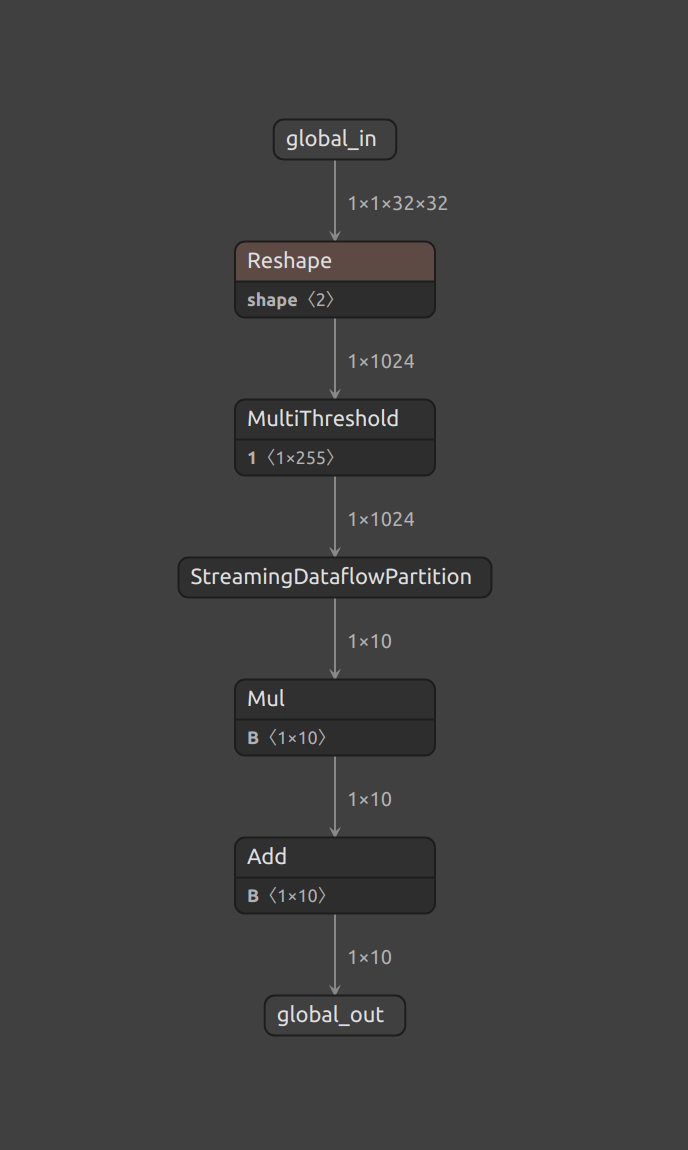
\includegraphics[width=6cm]{Figures/ONNXEnd.png}
	\caption[Transformed TFC \emph{ONNX} representation]{Transformed TFC \emph{ONNX} Representation}
	\label{fig:ONNXEnd}
\end{figure}

Once the graph is separated into two distinct parts, the synthesis can begin using \emph{Vivado}. Each layer is converted to one \emph{IP block}, a logical unit, then they are all stitched together to form the whole partition that will be ported to the board, as presented on \emph{Figure} \ref{fig:FINNSynthesis}. This part produces a \emph{bitfile} that defines the configuration of the FPGA.

% \emph{FINN} SYNTHESIS
\begin{figure}[htbp]
	\centering
		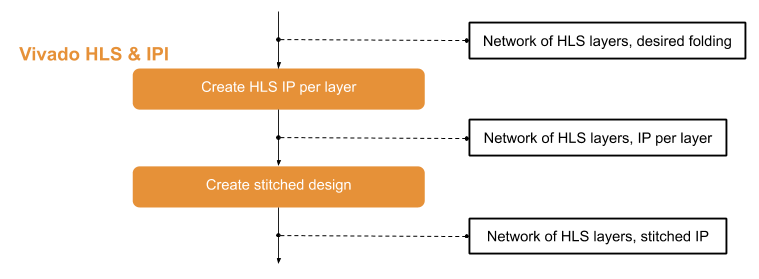
\includegraphics[width=10cm]{Figures/FINNSynthesis.png}
	\caption[FINN Synthesis]{FINN Synthesis}
	\label{fig:FINNSynthesis}
\end{figure}

Finally, the default built-in way to deploy the bitfile and execute it is to use the Python shield image named \emph{PYNQ}. This shield provides a Python environment to interact with the board. \emph{FINN} therefore creates and deploys a PYNQ project that consists of the base modules needed, a project structure and a simple driver. Once the project bitfile is transferred on the board, the driver can feed it with the image to inference, collect the result and send it back to the \texttt{onnx-exec} process. These different parts are summarised on \emph{Figure} \ref{fig:FINNPYNQ}.

% PYNQ DEPLOYMENT
\begin{figure}[htbp]
	\centering
		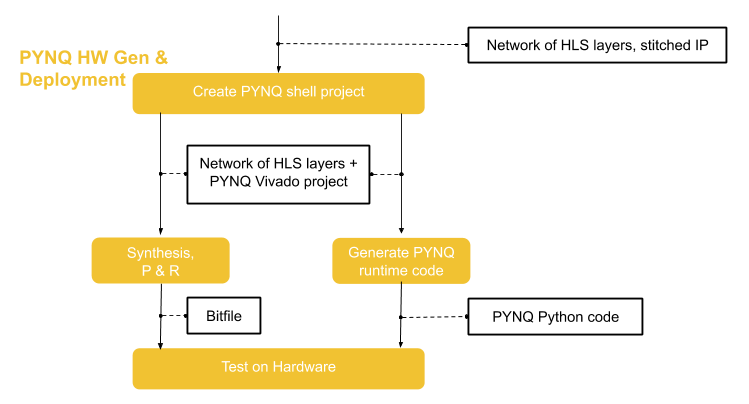
\includegraphics[width=10cm]{Figures/FINNPYNQ.png}
	\caption[FINN PYNQ Deployment]{FINN PYNQ Deployment}
	\label{fig:FINNPYNQ}
\end{figure}

%-------------------------------------------
%	SUBSECTION 6.2.4 - Benchmark as extension
%-------------------------------------------

\subsection{Benchmark as Extension}

The workflow \emph{Brevitas} / \emph{ONNX} / \emph{FINN} presents an interesting straightforward way to port a neural network on an FPGA board. In order to design a benchmark of the framework and to assess the impact of quantisation, there is a need for another layer on top of \emph{Brevitas} that should be able to train, evaluate and export neural networks. While Xilinx developers provide several examples to train and export different networks, they do not respect a common API nor the same structure rules. They are bundled in separate projects with instructions on how to run the training again but no insight is provided on what do hardcoded values mean on several quantised layers.

The different objectives of the benchmark are:
\begin{itemize}
  \item Present a common API to train neural networks, quantised or not.
  \item Be able to resume the training at any point.
  \item Log the different parts of the training.
  \item Define well-known neural networks and their quantised counterparts.
  \item Set an easy access to well-known datasets.
  \item Provide a common API to evaluate neural networks.
  \item Be able to export the trained neural network to \emph{ONNX}.
\end{itemize}

The project is structured as follows:
\begin{itemize}
  \item \textbf{\texttt{core}}: Core functionalities of the benchmark tool. This sub-package contains the \texttt{CLI}, \texttt{Trainer}, \texttt{Plotter}, \texttt{Logger} and \texttt{Exporter}. The \texttt{Trainer} is the main piece and is given all the arguments passed to the \texttt{CLI}. The \texttt{Logger} logs training routine, the \texttt{Plotter} allows to visualise instances of the dataset and the \texttt{Exporter} performs the export to \emph{ONNX}.
  \item \textbf{\texttt{extensions}}: Extensions of PyTorch functionalities to perform with quantised networks. These extensions consist of a new dataset, \emph{GTSRB}, a new loss function that can be used with binary networks, \emph{Squared Hinge Loss}, and a helper layer that performs the norm of the tensor.
  \item \textbf{\texttt{networks}}: Network architectures and their quantised counterpart. The defined networks consist of \texttt{TFC} ()three \emph{FC} layers next to each other), \texttt{CNV} (a simple CNN), \texttt{LeNet5}, \texttt{VGG11}, \texttt{VGG13}, \texttt{VGG16}, \texttt{VGG19} and \texttt{MobilenetV1}. All the different architectures answer to the same API and can be created by passing the number of \emph{classes}, number of \emph{in-channels} and the different quantisations if using a quantised network. The creation of a simple network and its quantised counterpart can be seen on \emph{Figure} \ref{fig:NetworkCreation}.
\end{itemize}

% PROJECT UML
% \begin{figure}[htbp]
% 	\centering
% 		\includegraphics[width=8cm]{Figures/BenchCLI.png}
% 	\caption[Benchmark CLI]{Benchmark Command Line Interface}
% 	\label{fig:BenchCLI}
% \end{figure}


\begin{figure}[htbp]
\centering
\begin{lstlisting}[language=Python]
from nn_benchmark.networks import LeNet5, QuantLeNet5

# To train a classic PyTorch network on MNIST for example
# (10 classes and black and white images)
lenet5 = LeNet5(n_classes = 10, in_channels = 1)

# To train a quantised \emph{Brevitas} network on CIFAR-10 for example
# (10 classes and RGB images) with quantisations of 2 bits for the
# weights, 2 bits for the activations and 4 bits for the first layer
quant_lenet5 = QuantLeNet5(n_classes = 10, in_channels = 3,
                           weight_bit_width = 2,
                           act_bit_width    = 2,
                           in_bit_width     = 4)
\end{lstlisting}
\caption[NetworkCreation]{Network Creation with the benchmark tool}
	\label{fig:NetworkCreation}
\end{figure}

The training routine is wrapped up by the \texttt{Trainer} class and can be tuned through the command line. The \texttt{CLI} class holds a large number of parameters that can be used to customise the training phase. An example of a run can be seen on \emph{Figure} \ref{fig:BenchCLI}. The example presented on the figure will launch the training for the network \texttt{QuantTFC}, the \emph{Brevitas} version of the \emph{TFC} network (three successive fully-connected layers). This training will be run on the \texttt{FashionMNIST} dataset for 100 epochs. It will be overlooked by the \texttt{ADAM} optimiser and \texttt{CrossEntropy} loss function. The hyper-parameters are tuned to a learning rate of 0.01 and a momentum of 0.9. The learning rate will change according to the scheduler, here a \texttt{MultiStepScheduler}. This scheduler will divide by 10 the learning rate after the epochs specified as milestones, here 34 and 37. Finally, the \emph{activation quantisation} is set to 2 bit, same for the \emph{weight quantisation} and the \emph{input quantisation} is set to 8 bits. The input quantisation is used for the first layer only. This often outputs better results due to the avoided harsh precision reduction. The first layers impact end accuracy a lot more than the last ones and the quantisation has to be delayed.

\begin{figure}[htbp]
\centering
\begin{lstlisting}[language=bash]
PYTORCH_JIT=1 python nn_benchmark/main.py \
--network    QuantTFC     \
--dataset    FashionMNIST \
--epochs     100          \
--optimiser  ADAM         \
--loss       CrossEntropy \
--lr         0.01         \
--momentum   0.9          \
--scheduler  STEP         \
--milestones 34,37        \
--acq        2            \
--weq        2            \
--inq        8
\end{lstlisting}
\caption[Command Line Interface]{Command Line Interface arguments}
	\label{fig:BenchCLI}
\end{figure}

The programs in \texttt{quant\_utils\/} present helper methods to create the different quantised layers. Those helpers work as both a simplification of the quantised layers API but also as controllers of the homogeneity of the layers functionalities. This homogeneity is crucial as, for now, \emph{FINN} can only handle a subset of what \emph{Brevitas} is able to design and train.

The final project can be seen on GitHub under the name \texttt{nn\_benchmark} \cite{BenchmarkRepo}.

%----------------------------------------------------------------------------------------
%	SECTION 6.3 - Methodology and Setup
%----------------------------------------------------------------------------------------

\section{Methodology and Setup}

This section will present the setup and methodology of the different experiments run. This is important for reproducibility purposes and to present results comparable to the literature. Those results aim at being extended in the future. \emph{FINN} and \emph{Brevitas} are not released yet and are still in development. The API of both tools is subject to change and results will need to be reassessed. However, the training part of the benchmark should not be subject to change as it uses a subset of the \emph{Brevitas} functionalities. While \emph{Brevitas} allows extensive tuning and customisation of both networks and training routine, \emph{FINN} can only (for now) handle a subset of those customisations.

%-----------------------------------
%	SUBSECTION 6.3.1 - Experiments
%-----------------------------------

\subsection{Experiments}

In order to assess the impact of quantisation, the objective is to deploy a neural network with varying precision for its weights and activations. The different metrics that will be taken in consideration are the following:

\begin{itemize}
  \item \textbf{Weight Bitwidth}: The number of bits in the weight precision.
  \item \textbf{Activation Bitwidth}: The number of bits in the activation precision.
  \item \textbf{Network Accuracy}: The final accuracy of the trained network on the test set.
  \item \textbf{Training Time}: Number of epochs the network was trained for.
  \item \textbf{Hardware Utilisation}: Look-up tables (LUT), flip-flops (FF) and BRAM usage.
  \item \textbf{Throughput}: Number of image the deployed network can process per second.
\end{itemize}

The initial objective was to train three different neural networks and their according datasets, the three being:
\begin{itemize}
  \item \textbf{TFC} for \textbf{Fashion-MNIST}: A simple neural network containing three fully-connected layers to train on a variation of the handwritten digits dataset, \emph{Fashion-MNIST} using small grayscale images of garments.
  \item \textbf{CNV} for \textbf{CIFAR-10}: A simple convolutional neural network to run on a classic 3-channels dataset, CIFAR-10.
  \item \textbf{MobilenetV1} for \textbf{GTSRB}: This network is interesting due to the fact it has been designed with portability in mind, coupling it with a street signs dataset makes it an interesting combination in an autonomous driving context.
\end{itemize}

%--------------------------------------
%	SUBSECTION 6.3.2 - Training
%--------------------------------------

\subsection{Training}

The training of the different networks is made with the following parameters and hyper-parameters:
\begin{itemize}
  \item \textbf{Epochs}: 40
  \item \textbf{Momentum}: 0.9
  \item \textbf{Learning Rate}: 0.01
  \item \textbf{Scheduler}: Multi-step scheduler, the learning rate is divided by 10 on epochs 34 and 37 as done in \cite{}.
  \item \textbf{Batch size}: 100 instances per batch.
  \item \textbf{Loss function}: The loss function used is \emph{Cross Entropy}.
  \item \textbf{Optimiser}: The optimiser use dis the \emph{ADAM} optimiser as it has been shown it is the most performing one when dealing with reduced precision \cite{Alizadeh2018}.
\end{itemize}

Along with those parameters, the bit-widths of weights and activations are taken from 2 to 32 bits. There are no differences here between the weights and activations. While \cite{Bacchus2020} differentiates the bit-widths, this functionality is still not fully supported in \emph{Brevitas} / \emph{FINN}. The inputs are either 8 bits (for sub-8bits weights and activations) or 32 bits (for 16 and 32-bits weights and activations). A summary of the bit-widths used follows:
\begin{itemize}
  \item \textbf{weights}: 2, 4, 8, 16, 32
  \item \textbf{activations}: 2, 4, 8, 16, 32
  \item \textbf{inputs}: 8, 8, 8, 32, 32
\end{itemize}

Rather than using the \emph{CLI} to specify the training configuration for each one of the neural networks as in \emph{Figure} \ref{fig:BenchCLI}, a running script is provided as presented in \emph{Figure} \ref{fig:TrainingScript}. This script emulates the \emph{CLI} by passing the specified parameters and hyper-parameters presented earlier but varying both the network architecture, dataset and the different bit-widths.

\begin{figure}[htbp]
\centering
\begin{lstlisting}[language=Python]
import sys
from nn_benchmark.core import ObjDict, Trainer
from nn_benchmark.networks import QuantTFC, QuantCNV, QuantMobilenetV1

if __name__ == "__main__":
    acq_list = [2, 4, 8, 16, 32]
    weq_list = [2, 4, 8, 16, 32]
    inq_list = [8, 8, 8, 32, 32]

    args = {'datadir': './data/', 'experiments': './experiments', 'dry_run': False,
            'log_freq': 10, 'evaluate': False, 'resume': None, 'detect_nan': False,
            'num_workers': 4, 'gpus': '0', 'batch_size': 100, 'lr': 0.01, 'optim': 'ADAM',
            'loss': 'CrossEntropy', 'scheduler': 'STEP', 'milestones': '34,37',
            'momentum': 0.9, 'weight_decay': 0, 'epochs': 40, 'random_seed': 1,
            'network': None, 'pretrained': False, 'dataset': None,
            'visualize': False, 'acq': None, 'weq': None, 'inq': None, 'onnx': False}
    args = ObjDict(args)

    # QuantTFC on Fashion-MNIST
    args.network = "QuantTFC"
    args.dataset = "FASHION-MNIST"
    for acq, weq, inq in zip(acq_list, weq_list, inq_list):
        args.acq = acq
        args.weq = weq
        args.inq = inq
        trainer_tfc = Trainer(args)
        trainer_tfc.train_model()

    # QuantCNV on CIFAR-10
    args.network = "QuantCNV"
    args.dataset = "CIFAR10"
    for acq, weq, inq in zip(acq_list, weq_list, inq_list):
        args.acq = acq
        args.weq = weq
        args.inq = inq
        trainer_cnv = Trainer(args)
        trainer_cnv.train_model()

    # QuantMobilenetV1 on GTSRB
    args.network = "QuantMobilenetV1"
    args.dataset = "GTSRB"
    for acq, weq, inq in zip(acq_list, weq_list, inq_list):
        args.acq = acq
        args.weq = weq
        args.inq = inq
        trainer_mobilenet = Trainer(args)
        trainer_mobilenet.train_model()
\end{lstlisting}
\caption[Training Script]{Training Script to train all three networks}
	\label{fig:TrainingScript}
\end{figure}

%--------------------------------------
%	SUBSECTION 6.3.3 - Deployment
%--------------------------------------

\subsection{Deployment}

The deployment step is performed through the different \emph{FINN} transformations. The target architecture is a \emph{PYNQ-Z1}, a Python shell over a circuit from the \emph{Zynq} family. The \emph{Zynq} circuits are composed of an \guille{Ap SoC} (All Programmable System-on-Chip) that contains a dual-core ARM Cortex-A9.

While the target here is the base shell holder\emph{PYNQ-Z1}, the Python shell can be ported to other architectures. For now, the official supported architectures are \emph{PYNQ-Z1} or \emph{PYNQ-Z2} from Digilent and \emph{ZCU104} or \emph{ZCU111} from Xilinx. However, instructions to create your own image are available and several community \emph{PYNQ} images are available (\emph{Avnet Ultra96} for example).

Looking through the transformations steps presented earlier, here are the transformations used:
\begin{itemize}
  \item \textbf{Tidy-up}: This first step calls different transformations to simplify the graph. The transformations used here are \texttt{DoubleToSingleFloat}, \texttt{InferShapes}, \texttt{FoldConstants}, \texttt{GiveUniqueNodeNames}, \texttt{GiveReadableTensorNames} and \texttt{InferDataTypes}.
  \item \textbf{Streamline}: The streamline process described earlier is resumed to the \texttt{Streamline} transformation.
  \item \textbf{HLS Conversion}: The conversion consists of changing the layers to their HLS counterpart. In the case of quantised FC layers, the transformation is \texttt{Infer} \texttt{QuantizedStreamingFCLayer}.
  \item \textbf{Dataflow Partition}: The separation is contained in the \texttt{CreateDataflowParti-} \texttt{tion} transformation.
  \item \textbf{Folding}: The tuning operates on the child containing the HLS layers of the previously created partition. This folding is an empiric process for now but can be guided using \guille{folding factors}. Here, the folding factor used was 32. Each image consists of 1024 pixels ($32 \times 32$) and the PE and SIMD determines the number of simultaneous operations that can be processed in order to process the full image. The higher the folding factor, the higher number of passes are needed but the fewer hardware resources used. The \emph{PYNQ} being a relatively small FPGA, a folding factor of 16 was too much to handle and therefore 32 is chosen. The folding process can be seen on \emph{Figure} \ref{fig:FoldingProcess}. After selecting the PE and SIMD, the transformations \texttt{InsertDWC} \texttt{InsertFIFO} and \texttt{InsertTLastMarker} can be used.

  \begin{figure}[htbp]
  \centering
  \begin{lstlisting}[language=Python]
  fc_layers = model.get_nodes_by_op_type("StreamingFCLayer_Batch")
  # (PE, SIMD, in_fifo_depth, out_fifo_depth, ramstyle) for each layer
  # Test Divided by two the PE and in_fifo_depth
  config = [
      (16, 64, 16, 64, "block"),
      (8, 8, 64, 64, "auto"),
      (8, 8, 64, 64, "auto"),
      (10, 8, 64, 10, "distributed"),
  ]
  for fcl, (pe, simd, ififo, ofifo, ramstyle) in zip(fc_layers, config):
      fcl_inst = getCustomOp(fcl)
      fcl_inst.set_nodeattr("PE", pe)
      fcl_inst.set_nodeattr("SIMD", simd)
      fcl_inst.set_nodeattr("inFIFODepth", ififo)
      fcl_inst.set_nodeattr("outFIFODepth", ofifo)
      fcl_inst.set_nodeattr("ram_style", ramstyle)
  \end{lstlisting}
  \caption[Folding Process]{Folding process on the different layers}
  	\label{fig:FoldingProcess}
  \end{figure}
  \item \textbf{IP Synthesis}: The IP are synthesised using \texttt{PrepareIP}, \texttt{HLSSynthIP}, \texttt{ReplaceVeri-} \texttt{logRelPaths} and \texttt{CreateStitchedIP}. The result is a stitched IP consisting of one IP per layer succeeding one another. The resulting block design is presented on \emph{Figure} \ref{fig:StitchedBlockDesign} and displays successive \texttt{StreamingFIFO} and \texttt{StreamingFCLayer\_Batch}.

  \newpage

  % VIVADO STITCHED PROJECT
  \begin{figure}[htbp]
  	\centering
  		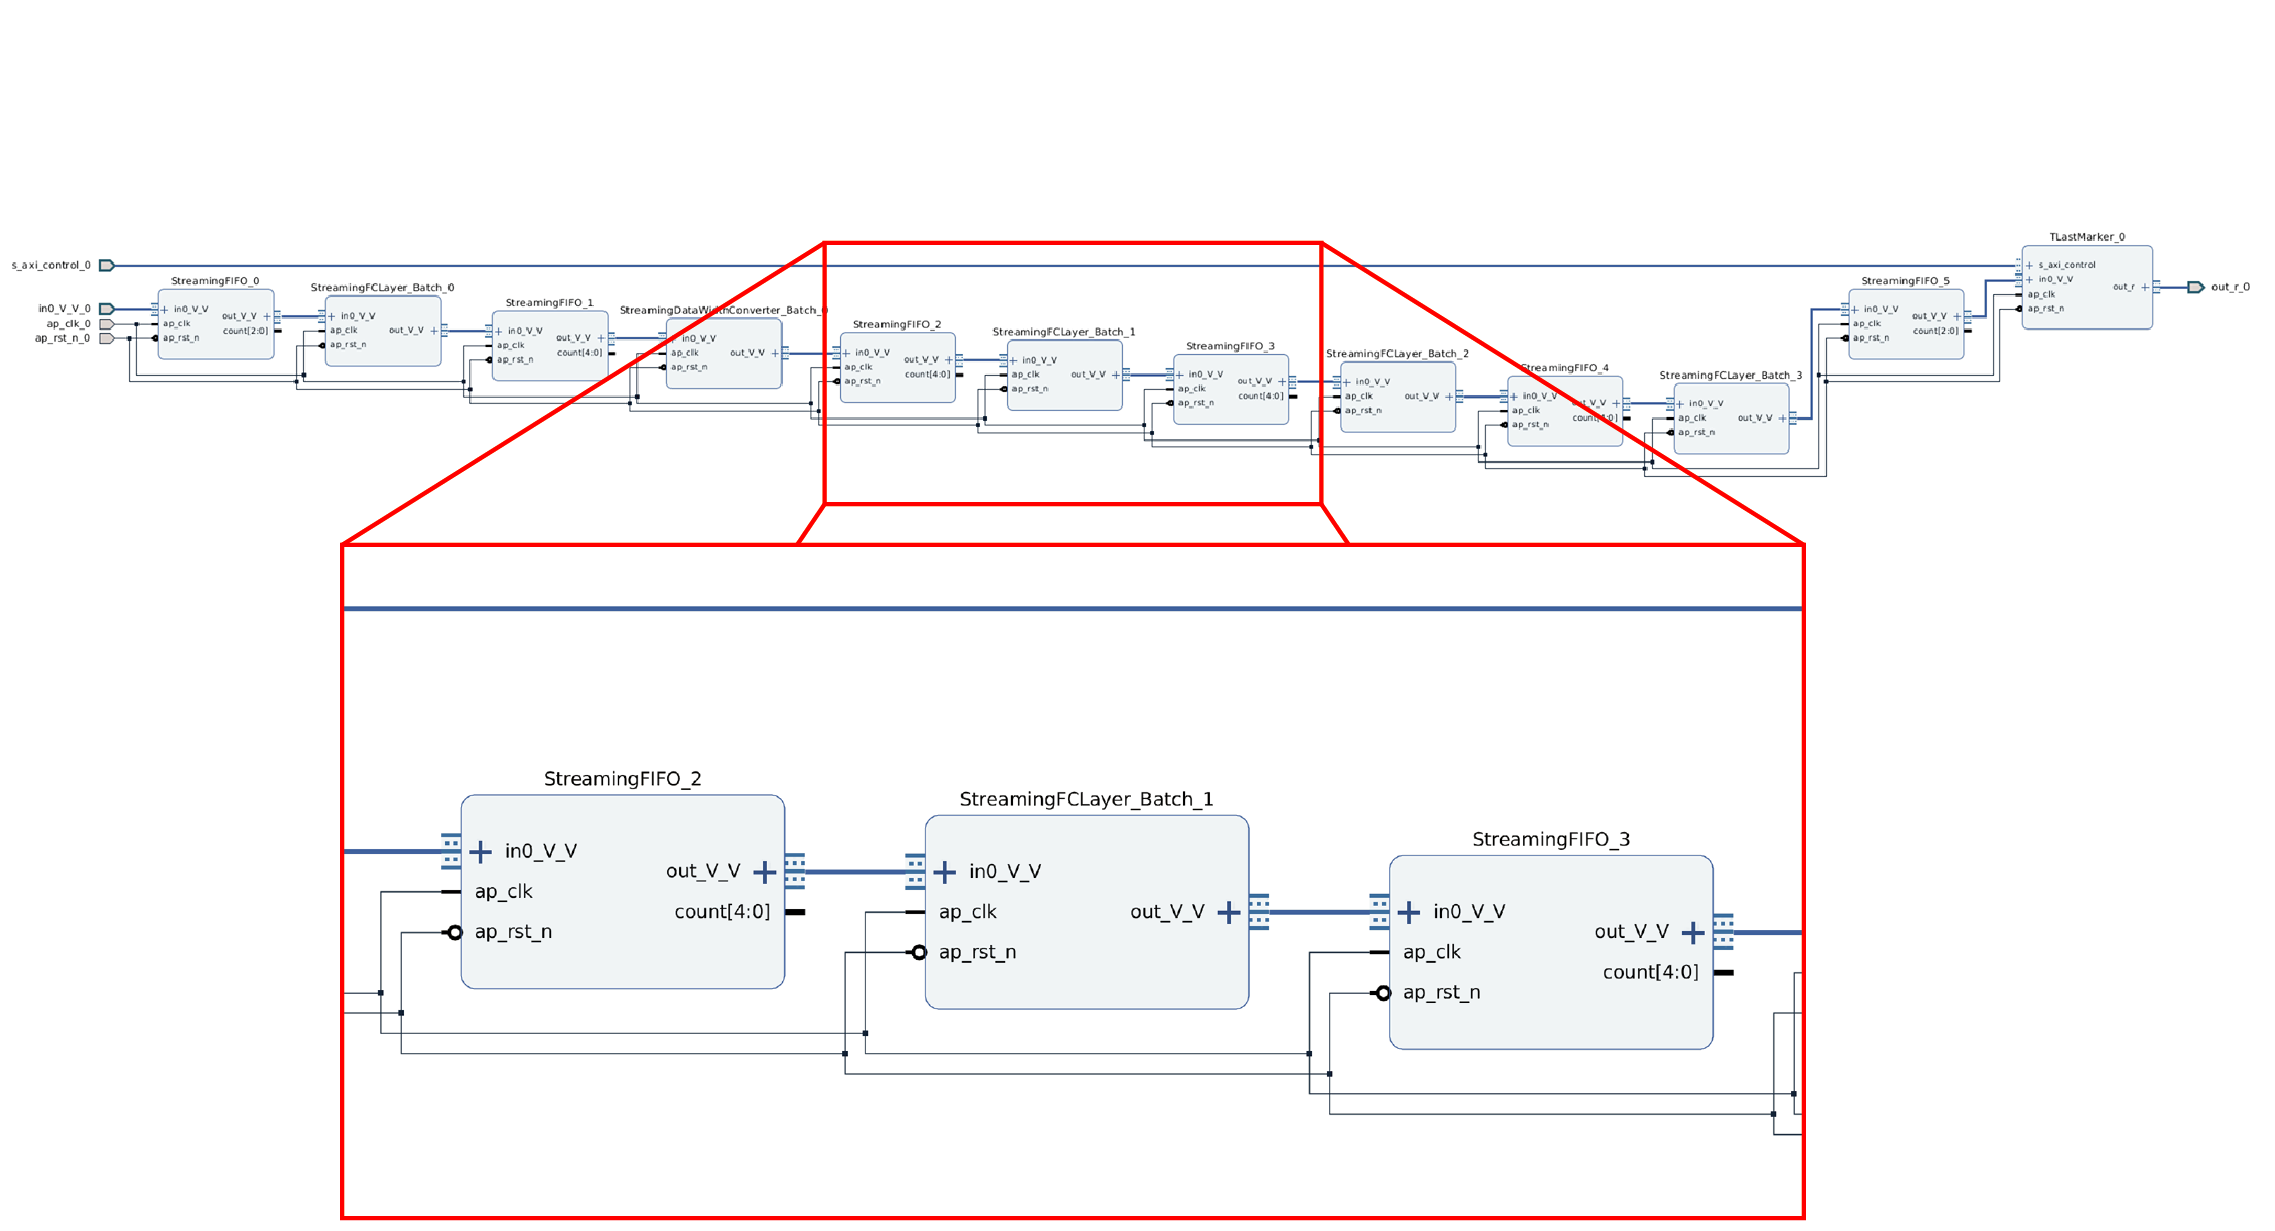
\includegraphics[width=\textwidth]{Figures/StitchedBlockDesign.png}
  	\caption[StitchedBlockDesign]{Block Design of the stitched IP layers}
  	\label{fig:StitchedBlockDesign}
  \end{figure}

  \item \textbf{PYNQ deployment}: The PYNQ driver and project are created with \texttt{Make-} \texttt{PYNQProject}, \texttt{SynthPYNQProject} and \texttt{MakePYNQDriver} and deployed with \texttt{DeployToPYNQ}.
\end{itemize}

These steps create a final \emph{Vivado} project, perform the synthesis and transfer the bitfile to the \emph{PYNQ-Z1}. An overview of the \emph{Vivado} block design can be seen on \emph{Figure} \ref{fig:ProjectBlockDesign}. The highlighted portion corresponds to the actual neural network part. The other components are links to the processing unit or external memory. A picture of the \emph{PYNQ-Z1} can be seen on \emph{Figure} \ref{fig:PYNQ-Z1}.

% FINAL VIVADO BLOCK DESIGN
\begin{figure}[htbp]
	\centering
		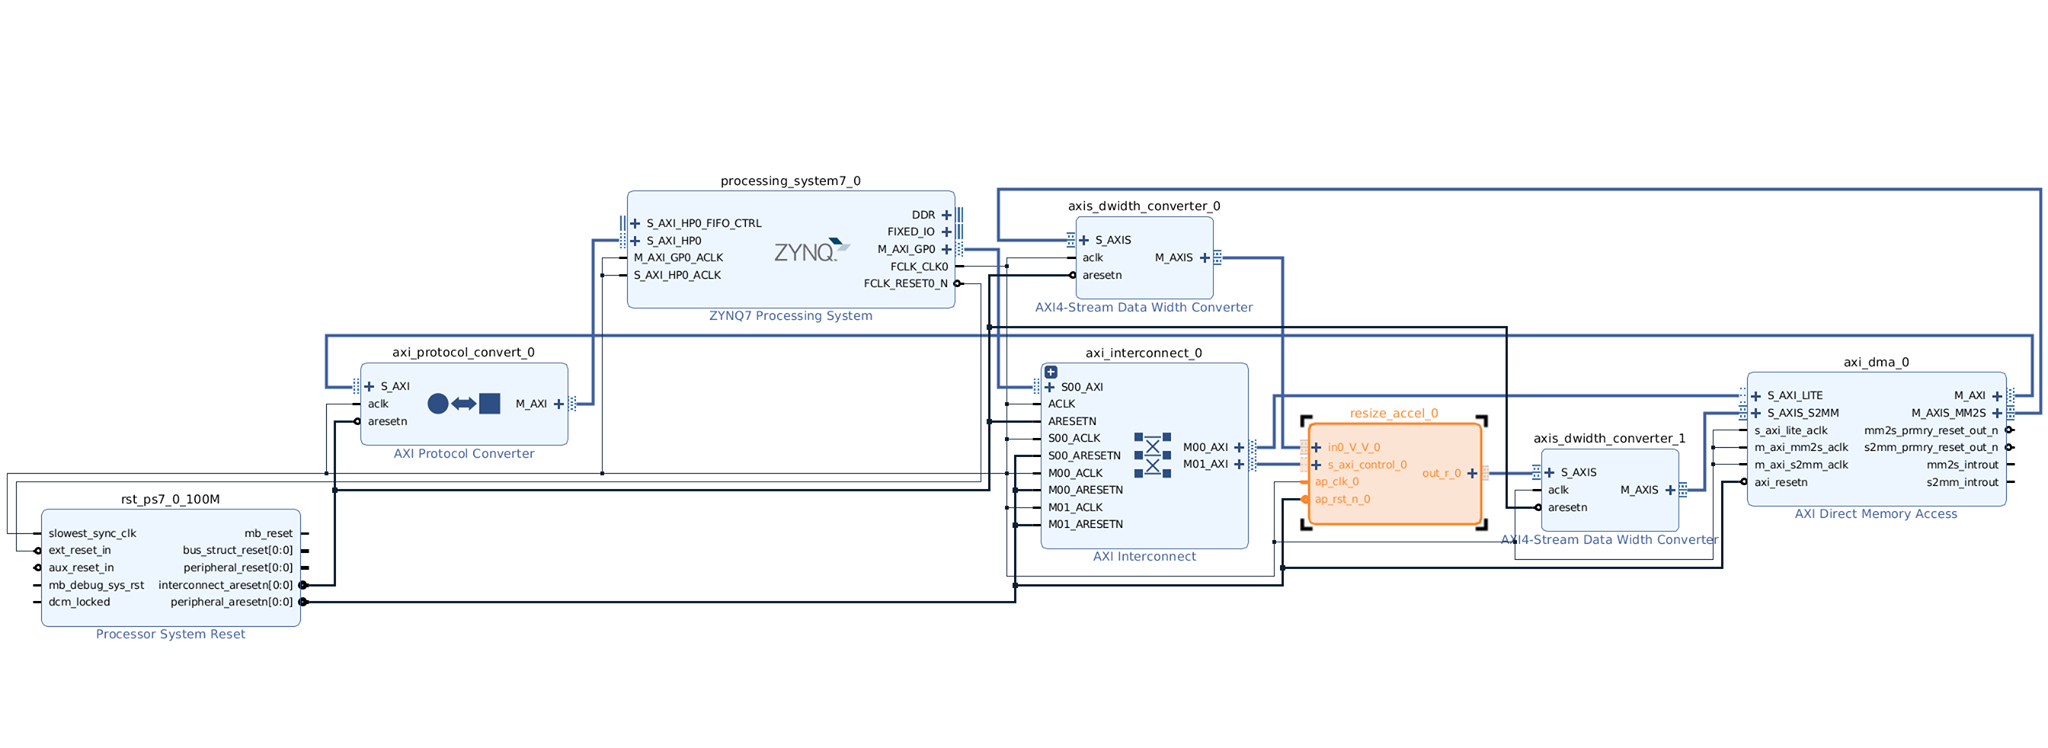
\includegraphics[width=\textwidth]{Figures/ProjectBlockDesign.png}
	\caption[ProjectBlockDesign]{Final Vivado Block Design}
	\label{fig:ProjectBlockDesign}
\end{figure}

% PYNQ PHOTO
\begin{figure}[htbp]
	\centering
		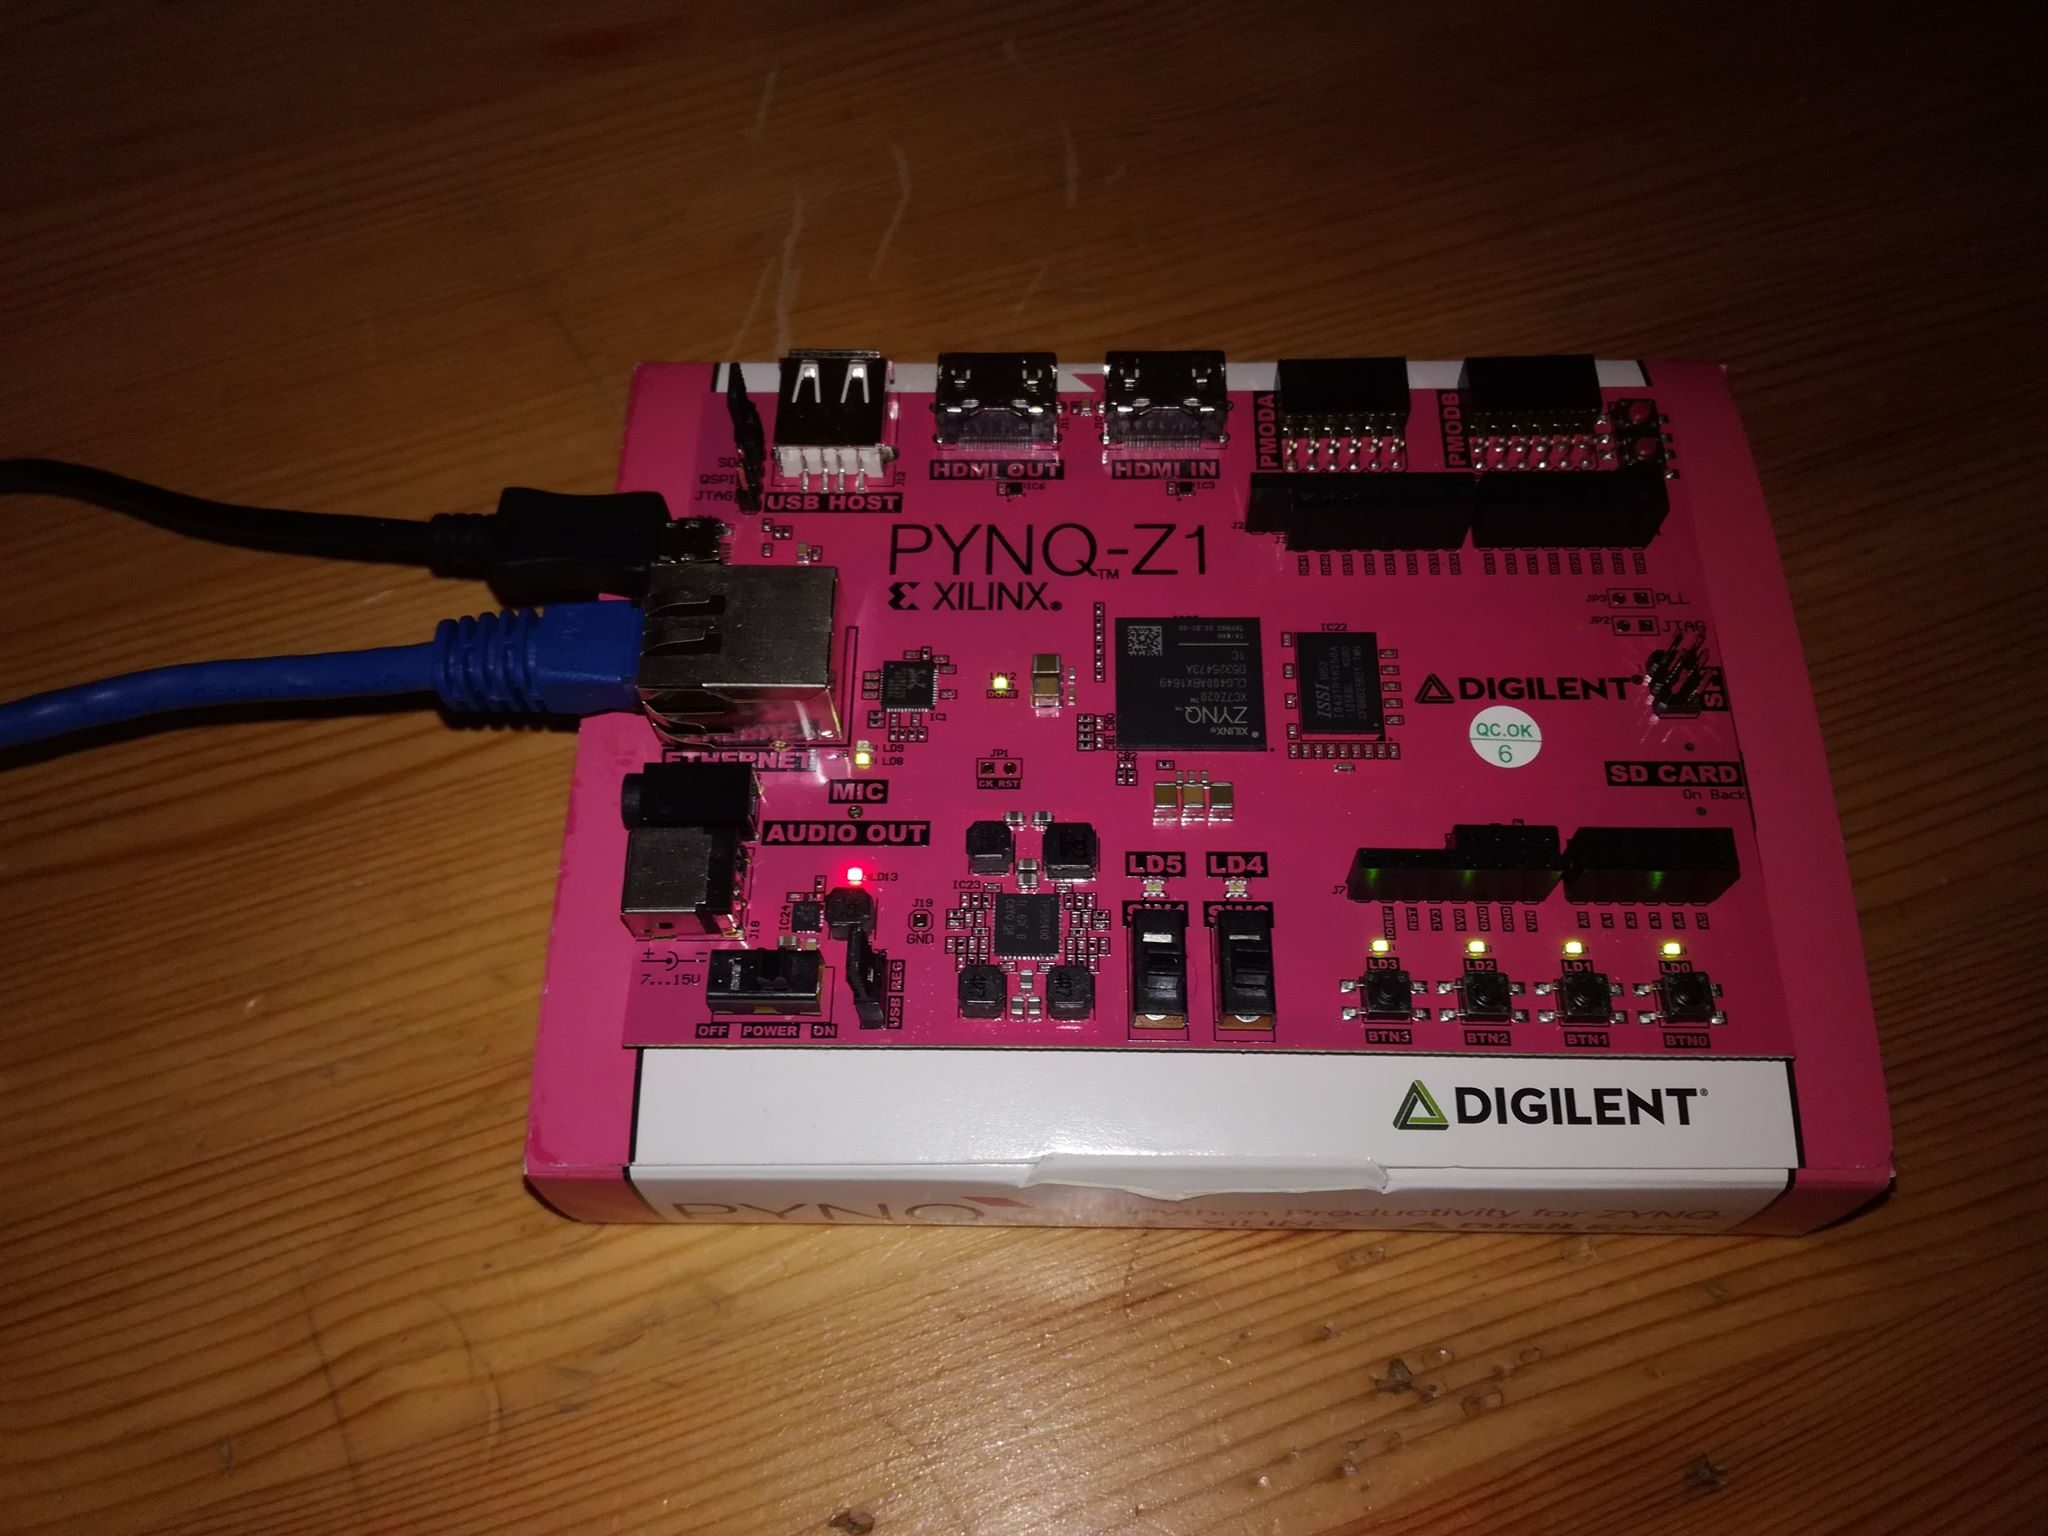
\includegraphics[width=\textwidth]{Figures/PYNQ.png}
	\caption[PYNQ-Z1]{PYNQ-Z1 with a neural network deployed}
	\label{fig:PYNQ-Z1}
\end{figure}


\newpage

In the end, it is possible to provide an image to the deployed network as presented on \emph{Figure} \ref{fig:DeployedInference}. This figure presents a script to first load the image and convert it to a tensor. Then, the trained transformed network is loaded and \texttt{onnx-exec} is used to run the image through the network. The result is then interpreted through the \texttt{softmax} function that outputs the different probabilities of each class for the provided picture.

\begin{figure}[htbp]
\centering
\begin{lstlisting}[language=Python]
import numpy as np
from \emph{FINN}.core.onnx_exec import execute_onnx
# Loading the image
image = Image.open('/workspace/finn/onnx_experiments/img_MNIST.png')
x = TF.to_tensor(image)
x.unsqueeze_(0)
# Loading the parent model of the partition
parent_model = load("dataflow_parent")
sdp_node = parent_model.graph.node[2]
remote_exec_model = build_dir + "tfc_deploy.onnx"
getCustomOp(sdp_node).set_nodeattr("model", remote_exec_model)
save(parent_model,"dataflow_parent_with_remote_bitfile_exec")
# Running the model, the deployed part will go to the FPGA once the node is reached
iname = parent_model.graph.input[0].name
oname = parent_model.graph.output[0].name
ishape = parent_model.get_tensor_shape(iname)
input_dict = {iname: x.numpy()[0].reshape(ishape)}
ret = execute_onnx(parent_model, input_dict, True)
# Definition of the softmax function
def softmax(x):
    """Compute softmax values for each sets of scores in x."""
    e_x = np.exp(x - np.max(x))
    return e_x / e_x.sum()
logits = ret[oname].flatten()
prob = softmax(logits)
# Presentation of the probabilities for the given image
plt.bar(np.arange(10), prob)
\end{lstlisting}
\caption[Deployed Inference]{Inference on the deployed network}
  \label{fig:DeployedInference}
\end{figure}

Moreover, \emph{FINN} provides a way to conduct a throughput test as presented on \emph{Figure} \ref{fig:ThroughputTest}. The test takes advantage of \emph{FINN} function \texttt{throughput\_test} that outputs both the throughput and other i/o metrics such as the DRAM bandwidth for example.

\begin{figure}[htbp]
\centering
\begin{lstlisting}[language=Python]
from \emph{FINN}.core.throughput_test import throughput_test

child_model = ModelWrapper(getCustomOp(sdp_node).get_nodeattr("model"))
res = throughput_test(child_model)
print("Network metrics:")
for key in res:
    print(str(key) + ": " + str(res[key]))
\end{lstlisting}
\caption[Throughput Test]{Throughput test method}
  \label{fig:ThroughputTest}
\end{figure}
